\section{Discussion}

% 我们定义以下符号以支持形式化推导：
% \begin{itemize}
%     \item $S_t$: 在 $t$ 时刻的状态，S_i代表第i个位置的token是S_i。
%     \item $M_t$: t时刻的掩码位置集合。
%     \item $A_t$: t时刻决定要解码的位置集合。
%     \item H_t,代表历史解码位置集合。H_t[i]代表第i步解码的位置的集合
%     \item $PH(H_t) = \sum_i^t\sum_{j}^{j\in A_i} H(P_j^t)$: 定义为路径概率（Path Probability），
%     \item $U(S_t)$: 定义为状态 $S_t$ 下的效用函数。
%     U_{m,pi}(S_t) = $Argmax_{H\sim D(m,\pi,S_t)}(PH(H_n))$，其中H_n是终态，所有的掩码都被解除了。D(m,\pi,S_t)代表利用model m和policy \pi来进行采样的,以S_t为初始状态所采样得到的历史解码路径。
% \end{itemize}

% \section{Problem Formalization}
% 优化的核心难题在于目标状态 $S_n$ 的Argmax效用难以直接获取。
% 因此，我们引入立即解码（Immediate Decoding）作为替代策略。它指的是把当前剩余的掩码全部解码了。
% \begin{equation}
%     H_{ind}(m, \pi, H_t) = H(H_t) + H(\dots) \text{ [cite: 27]}
% \end{equation}
% 注意：立即解码是DLM独有的好处，ARM必须自回归完成才能得到一个路径熵。
% \section{Analysis of Scale Bias}
% 由于立即解码策略和真实采样策略存在差异，会产生 Scale 上的偏差。我们需要引入\alpha来近似这个误差：
% U_{m,\pi'} = U_{m,\pi} * \alpha(t)
% 其中t是真实解码策略所采样解码剩余掩码的步数。
% 我们通过实际实验测算出\alpha（t）是一个有界的函数。随着t增大，\alpha(t)从1增加到某一个上限B。类似S形曲线
% 接下来，我们给出，在当前状态为S_t是，选择动作A_t所带来的信息增益。
% 在动作选择 $A_t$ 时，我们考虑增量更新 $\Delta U$：
% \begin{equation}
%     \text{argmin } \Delta U =
%     U_{m,\pi}(S_{t+1})-U_{m,\pi}(S_t)
%     =\sum_{i\in A_i}H(P_i^t)+\frac{\sum_{i\in{M_t-A_t}H(P_i^{t+1})}{\alpha(N-t-1)}-\frac{\sum_{i\in{M_t}H(P_i^{t})}{\alpha(N-t)}
%     = (1-\frac{1}{\alpha(N-t)})\sum_{i\in M_t}H(P_i^t)+\frac{\sum_{i\in{M_t-A_t}H(P_i^{t+1})}{\alpha(N-t-1)}-\frac{\sum_{i\in{M_t-A_t}H(P_i^{t})}{\alpha(N-t)}
% \end{equation}
% 第一项是greedy entropy target, 第二项是future informatin gain.
\subsection*{Mathematical Notations}

To support the formal derivation, we define the following notations:

\begin{itemize}
    \item $S_t$: The state at time $t$, defined by the current configuration of tokens and masks.
    \item $M_t$: The set of indices of currently masked positions.
    \item $A_t \subseteq M_t$: The action taken at time $t$, representing the set of positions chosen to be decoded.
    \item $H_n = \{A_1, A_2, \dots, A_n\}$: A complete decoding trajectory (history) resulting in a terminal state where $M_n = \emptyset$.
    \item $PH(H_t) = \sum_{i=1}^t \sum_{j \in A_i} H(P_j^i)$: The \textbf{Path Entropy}, representing the cumulative entropy of all positions decoded up to time $t$.
    \item $U(S_t)$: The \textbf{Utility Function}, representing the expected total path entropy from state $S_t$ to the terminal state:
    \begin{equation}
        U(S_t) = \mathbb{E}_{H_n \sim D(m,\pi,S_t)} [PH(H_n)]
    \end{equation}
    \item $Q(S_t, A_t)$: The \textbf{Action-Value Function}, representing the expected cumulative entropy if action $A_t$ is taken at state $S_t$ and policy $\pi$ is followed thereafter:
    \begin{equation}
        Q(S_t, A_t) = \sum_{j \in A_t} H(P_j^t) + \mathbb{E}[U(S_{t+1}) | S_t, A_t]
    \end{equation}
\end{itemize}

\subsection{Optimization Objective}
Our objective is to find an optimal decoding trajectory $H_n^*$ that minimizes the total Path Entropy $PH(H_n)$. Formally, at any state $S_t$, the problem is equivalent to finding the optimal action $A_t^*$ that minimizes the $Q$-value:
\begin{equation}
    A_t^* = \argmin_{A \subseteq M_t} Q(S_t, A)
\end{equation}

\subsection{Problem Formalization via Immediate Decoding}
The exact computation of $Q(S_t, A_t)$ is intractable as it requires marginalizing over all possible future decoding paths. In Discrete Diffusion Language Models (DLMs), we can approximate future utility using \textbf{Immediate Decoding} ($H_{\text{ind}}$), which assumes all remaining masks $M_{t+1}$ are decoded in a single parallel step.

To correct the systematic scale bias between immediate decoding and true sequential sampling, we introduce a correction factor $\alpha(k)$:
\begin{equation}
    \hat{U}(S_t) = \frac{1}{\alpha(k)} \sum_{j \in M_t} H(P_j^t)
\end{equation}
where $k = |M_t|$ is the number of remaining masks. Experimentally, $\alpha(k)$ is an S-shaped bounded function where $\alpha(1)=1$ and $\lim_{k \to N} \alpha(k) = B$.

\subsection{Analysis of the One-Step Beam Search Planner}
By substituting the scaled estimator $\hat{U}$ into the definition of $Q(S_t, A_t)$, the optimal action $A_t$ is chosen to minimize the incremental change in expected total entropy, $\Delta U$:

\begin{equation}
\begin{aligned}
    \Delta U(S_t, A_t) &= Q(S_t, A_t) - U(S_t) \\
    &\approx \left( \sum_{i \in A_t} H(P_i^t) + \hat{U}(S_{t+1}) \right) - \hat{U}(S_t) \\
    &= (1-\frac{1}{\alpha(N-t-1)})\sum_{i \in A_t} H(P_i^t) + \frac{\sum_{i \in M_{t+1}} H(P_i^{t+1})}{\alpha(N-t-1)} - \frac{\sum_{i \in M_t} H(P_i^t)}{\alpha(N-t)}
\end{aligned}
\end{equation}

By decomposing the current total entropy $\sum_{i \in M_t} H(P_i^t)$ into the decoded part $\sum_{i \in A_t} H(P_i^t)$ and the remaining part $\sum_{i \in M_{t+1}} H(P_i^t)$, we obtain the final decision objective:

\begin{align}
    \Delta U &\approx \underbrace{\left( 1 - \frac{1}{\alpha(N-t)} \right) \sum_{i \in A_t} H(P_i^t)}_{\text{Greedy Entropy Penalty}} +\\ &\underbrace{\left( \frac{\sum_{i \in M_{t+1}} H(P_i^{t+1})}{\alpha(N-t-1)} - \frac{\sum_{i \in M_{t+1}} H(P_i^t)}{\alpha(N-t)} \right)}_{\text{Future Information Gain}}
\end{align}

\textbf{Conclusion:} The one-step beam search serves as a robust planner by balancing the immediate entropy cost against the future information gain (reduction in uncertainty of remaining tokens), accurately adjusted by the empirical scale factor $\alpha$.

\jd{
Comments:
\begin{enumerate}
    \item What is $P_i^t$?
    \item A lot of mathematical jargon and notations that are introduced one-time. Better to contextualize everything using $H(\cdot)$
    \item MDP/Q-function formulation: Unnecessary to introduce $U(S_t)$ and $Q(S_t, A_t)$ and RL-style planning if we not abandoning exact Bellman equations and replacing them with ``Immediate Decoding'' approximation.
    \item Where does the immediate decoding argument come from? In a masked dLM, we don't have a single consistent joint distribution over the full masked tokens; \textbf{we only have conditionally-independent token marginals predicted by the denoiser}.  It is iffy for the whole argument to rest on the assumption that we decode all remaining masks in a single parallel step.
    \item Path entropy is not the MAP objective, see below.
    \item The $\alpha(k)$ scale correction is kinda dangerous: There is no closed form derivation that $\sum H(P_j^t)$ (greedy entropy) is proportional to expected future path entropy, let alone that the proportionality depends on $k$. You are using the mean-field entropy, i.e., $\sum_{i \in M_t} H(X_i \mid S_t)$ to approximate the joint entropy, i.e., $H(X_1,...,X_j \mid S_t)$  for $X_1, \dots, X_j \in M_t$. The correlation depends on the KL divergence (total correlation), i.e., $D_{KL} (p(X_1,...,X_j \mid S_t) \| \prod_i H(X_i \mid S_t))$. Assume $\alpha(k)$, a function of time seems wrong... it assumes homogenous scaling across different context (task) and states.  Moreover, \textbf{if you fit $\alpha$ empirically, the analysis becomes circular; you can fit $\alpha$ to make any heuristic argument look consistent...}
\end{enumerate}
If you want an argument that IGP is related to beam search, here is the rough skeleton I would follow:
\begin{enumerate}
    \item Show that one-step greedy/IGP performs approximate MAP decoding
    \item dLMs > ARM: Show the strength of one-step information gain in dLMs due to the ability to calculate marginals over all unmasked tokens whereas ARMs need K-step approximation to reduce uncertainty.
\end{enumerate}
}

\jd{random verbal vomit below, not fully fleshed out, a lot of contextualization cos i needed to remind myself of the algorithm so might double count with your previous writing}
\subsection{Relation between IGP and Beam-Search}

\subsubsection{Warmup: Beam Search in Autoregressive Language Modeling}
For an autoregressive model over sequences $X_{1;T}$,
\begin{align}
    p_\theta(X_{1:t}) = \prod_{t=1}^Tp_\theta(X_t|X_{<t})
\end{align}
The maximum a posteriori (MAP) decoding objective for autoregressive text generation aims to find the most probable trajectory, $\argmax \log p_\theta(X_{1:t})$. However, exhaustive search to find the globally optimal sequence is not tractable as it requires marginalizing over all possible future decoding paths.

A \textbf{greedy algorithm} that selects the best token candidate at each time step, i.e., $X_t = \argmax \log p_\theta(X_t|X_{<t})$, makes
a sequence of locally optimal decisions, but can lead to a globally sub-optimal sequence.

Beam search is a commonly-used heuristic in natural language processing to approximate MAP decoding. It is described as a pruned breadth-first search that keeps the top $K$ hypotheses by accumulating score under a scoring function (e.g., normalized cumulative sum of log probabilities) and expanding them. \emph{For brevity and due to the ubiquity of beam search literature, exact notations are not introduced here.}



\subsubsection{Information-Structure Difference}
In autoregressive decoding, at time $t$, we only have $p_\theta(X_{t+1}|X_{\leq t})$. One cannot directly observe the effect of choosing $X_{t+1}$ on uncertainty/entropy of tokens several positions ahead without rolling forward. As such, beam search in autoregressive models benefits from deeper tree search by maintaining a $K$-sized buffer and scoring over longer horizons (usually with some horizon-dependent penalty) to hedge against delayed effects.

In masked diffusion, due to the absence of the assumption of an autoregressive causal order, future uncertainty is not hidden behind a causal factorization. One can \textbf{obtain updated conditional distributions for all remaining unmasked positions} immediately after committing to a candidate action $A_t$. This one-step re-evaluation exposes long-range effects immediately; hence shallow beam search over actions can approximate mode-seeking behavior with far less search depth than autoregressive decoding.

\subsubsection{MDM Sampling as One-Step Beam Search}
\jd{Will fill in if we decide to implement beam search for diffusion sampling. Intuition: you have a K-sized buffer that you prune every decoding step.}

\subsubsection{IGP as One-Step Beam Search}
We begin by defining some notations:
\begin{itemize}
    \item $S_t$: The state at time $t$, defined by the current configuration of tokens and masks.
    \item $M_t$: The set of indices of currently masked positions.
    \item $A_t \subseteq M_t$: The action taken at time $t$, representing the set of positions chosen to be decoded.
\end{itemize}

The decoding target of a masked diffusion language model is a fully unmasked sequence $S_T$ obtained after repeated applications of the denoiser and planner. The model induces an distribution over terminal sequences conditioned on an initial masked template $S_0$ (and optionally a prompt). The marginal MAP decoding objective is
\begin{align}
S_T^\star &= \argmax p_\theta(S_T \mid S_0) \\ &=\argmax \sum_{S_{1:T-1}}\sum_{A_{0:T-1}} p_\theta(A_{0:T-1} \mid S_0) \prod_{t=0}^{T-1} p_\theta (S_{t+1} \mid S_t, A_t)
\end{align}
\jd{need double check the RHS factorization, needa sum over all combinations of actions and states.}
where $p_\theta(S_T\mid S_0)$ is implicitly defined by the iterative denoising transitions and intermediate sampling decisions, rather than by a left-to-right factorization in autoregressive models. Similarly, exact MAP search remains intractable.

Although the joint posterior over remaining masked tokens is not accessible, the denoiser provides marginal conditional probabilities $p_\theta(x_i \mid S_t), \; i\in M_t$. A natural global uncertainty proxy at state $S_t$ is the mean-field entropy
\begin{align}
\tilde H(S_t) = \sum_{i\in M_t} H\left(p_\theta(x_i \mid S_t)\right).
\end{align}
Intuitively, smaller $\tilde H(S_t)$ indicates that the posterior over completions has become more concentrated (more ``mode-like''). Making $\tilde H(S_t)$ small quickly aligns with approximate MAP (mode-seeking) decoding.


\subsubsection{Why IGP Improves Upon Greedy Entropy (SetSa-style) Planners}
Greedy entropy-based methods (Select-then-Sample) choose positions based on current marginal uncertainty, e.g.,
\begin{align}
I_t^{\text{greedy}} \in \argmin_{I\subseteq M_t,\ |I|=K}\sum_{i\in I} H\left(p_\theta(x_i \mid S_t)\right),
\end{align}
and then sample token values for $i\in I_t^{\text{greedy}}$. This policy is myopic; it optimizes the entropy of the \emph{selected positions} rather than the entropy of the \emph{remaining problem} after committing an action.

In contrast, IGP explicitly evaluates the downstream effects on the remaining uncertainty before committing to an action.

\jd{\emph{Sketch}}
Consider the expected one-step reduction in mean-field uncertainty from committing to an action $A_t$ at time $t$:
\begin{align}
    \Delta_{MF}(A_t) := \tilde H(S_t) - \mathbb{E}_{A_t} \Big[ \sum_{i\in M_t, i \notin A_t} H(X_i | S_t, A_t)\Big]
\end{align}
By the definition of conditional mutual information,
\begin{align}
    H(X_i \mid S_t) - \mathbb{E}_{A_t}\Big[H(X_i \mid S_t, A_t)\Big] = I(X_i;A_t \mid S_t)
\end{align}
\jd{Note that this $I$ is mutual information term. Also, we should not use $I$ for the selected indices in greedy entropy (i.e., Section 3.1.2), especillay if u are writing a information-theoretic paper, $I$ and $H$ are often reserved.}
Hence,
\begin{align*}
    \Delta_{MF}(A_t) = \sum_{i \notin A_t}I(X_i; A_t\mid S_t).
\end{align*}
Greedy entropy selection chooses $A_t$ by minimizing local entropy $H(A_t|S_t)$, which is not aligned with $\Delta_{MF}$. One only has the loose bound $I(X_i; A_t \mid S_t) \leq H(A_t \mid S_t)$. In fact, local-entropy minimization can be arbitrarily bad for global reduction because there exists models where $H(A_1\mid S_t)$ is low but yet $A_1$ is independent (provides no information) of the other unmasked tokens, giving $\Delta_{MF}(A_t) = 0$. Meanwhile, another action $A_2$ has higher entropy but determines many remaining tokens, yielding $\Delta_{MF}(A_2)$ arbitrarily large. Thus, ``picking the easiest token'' does not help to collapse global uncertainty.

On the other hand, IGP directly incorporates $\Delta_{MF}$ by calculating $\sum_{i\in M_t, i \notin A_t} H(X_i | S_t, A_t)$ for each $A_t \in \mathcal{C}$ \jd{(following your past notation here but ideally we wanna reduce notation, i.e., $\mathcal{C}$)}. Therefore IGP targets the correct information-theoretic quantity governing \textbf{one-step mean-field uncertainty reduction}.



\clearpage

\subsection{Scratch: Limitations of Token-Level Heuristics}

\noindent\textbf{Thought experiment.}  
Consider the following idealized scenario: an MDM $m$ must generate three numbers \(a\), \(b\), and \(c\). They are sampled from a data generating process whereby a and b are uniformly distributed and \(c = a \times b\).  
Let:
\begin{itemize}
    \item \(a\) and \(b\) be expressed in base \(x\), so each digit token is drawn from an alphabet of size \(x\);
    \item \(c\) be expressed in base \(y\), so each digit token is drawn from an alphabet of size \(y\).
\end{itemize}
Assume the model is \emph{ideal}—it perfectly captures the joint distribution of all valid triples \((a,b,c)\).

Before any tokens are generated, each digit position for (a,b) has a uniform distribution over its alphabet.  The digit positions for c will have equal or lower entropy (for example, the most significant bit will usually be 0). Thus the per‑digit entropy for \(a\) and \(b\) is
\begin{equation}
H_{\text{digit}}(a)=H_{\text{digit}}(b)=\log x,
\end{equation}
while for \(c\) it is
\begin{equation}
H_{\text{digit}}(c)\le\log y .
\end{equation}
Multiplication is conjectured to be computationally one‑way: given \(a\) and \(b\), computing \(c\) is easy, but recovering \(a\) and \(b\) from \(c\) (factorization) is hard. Consequently, the \emph{logical generation order} should be \(a,b \to c\): the factors must be determined before their product.

Now suppose the output bases satisfy \(y < x\). Then
\begin{equation}
H_{\text{digit}}(c) < H_{\text{digit}}(a),\, H_{\text{digit}}(b).
\end{equation}
If a scheduling heuristic selects the next position to decode by minimizing local entropy, it will prioritize digits of \(c\) before digits of \(a\) or \(b\). This leads to a contradiction: the model would attempt to generate the product \(c\) before knowing its factors \(a\) and \(b\), violating the logical dependency imposed by the multiplication constraint.
\begin{quote}
\textbf{Observation.} 
Local token-level probability metrics, such as entropy as well as confidence or confidence margin, are unreliable heuristics for decoding order because they reflect only syntactic uncertainty, not logical dependencies. 
This limitation persists even the MDM is ideal after pre-training.
\end{quote}
% % We can include the formal derivation of our method here.


% \subsection{Notation and Formalization}

% Let the decoding process involve the following mathematical objects:

% \begin{itemize}
%     \item \textbf{Position set}: $M = \{1, 2, \dots, m\}$, where $m$ is the total number of positions to be decoded
%     \item \textbf{Vocabulary}: $V = \{1, 2, \dots, n\}$, where $n = |V|$ is the vocabulary size
%     \item \textbf{Probability distribution}: $p_i \in \Delta^{n-1}$ represents the token probability distribution at position $i \in M$, where $\Delta^{n-1}$ is the $(n-1)$-dimensional probability simplex
%     \item \textbf{Entropy function}: $H(p) = -\sum_{j=1}^{n} p[j] \log p[j]$, where $p[j]$ denotes the probability of token $j$
%     \item \textbf{Action space}: $\mathcal{A} = M \times V$, the set of all possible position-token pairs
%     \item \textbf{State}: $S = \{p_i\}_{i \in M}$, representing the current decoding state with all position distributions
%     \item \textbf{Updated state}: $S'(i,j)$ denotes the state after executing action $(i,j)$, where token $j$ is fixed at position $i$
% \end{itemize}

% \subsection{Traditional Decoding Strategy}

% The traditional strategy follows a two-stage sequential decision process:

% \begin{enumerate}
%     \item \textbf{Position selection}: Choose the optimal position based on a local scoring function $f: \Delta^{n-1} \to \mathbb{R}$:
%     \begin{equation}
%         i^* = \arg\max_{i \in M} f(p_i)
%     \end{equation}
    
%     Common choices for the scoring function $f$ include:
%     \begin{align}
%         f_{\text{entropy}}(p) &= -H(p) \\
%         f_{\text{max}}(p) &= \max_{j \in V} p[j] \\
%         f_{\text{margin}}(p) &= \max_{j \in V} p[j] - \operatorname{second\_max}_{j \in V} p[j]
%     \end{align}
    
%     \item \textbf{Token sampling}: Sample a token from the selected position's distribution:
%     \begin{equation}
%         j^* \sim p_{i^*}
%     \end{equation}
% \end{enumerate}

% The computational complexity of this approach is $O(1)$ forward passes, requiring only one forward pass to obtain all distributions $\{p_i\}_{i \in M}$.

% \subsection{Equivalent Form of Traditional Strategy}

% The traditional strategy can be equivalently formulated as:

% \begin{enumerate}
%     \item \textbf{Independent token sampling}: For each position $i \in M$, sample a candidate token:
%     \begin{equation}
%         \forall i \in M, \quad j_i \sim p_i
%     \end{equation}
    
%     \item \textbf{Position selection}: Select the optimal position using the same scoring function:
%     \begin{equation}
%         i^* = \arg\max_{i \in M} f(p_i)
%     \end{equation}
% \end{enumerate}

% The key observation is that this formulation reveals a fundamental limitation: the decision at step 2 depends solely on $f(p_i)$, completely ignoring information about the specific token values $j_i$.

% This leads to a critical decoupling between decision and execution, which can be analyzed through two sources of error:

% \begin{enumerate}
%     \item \textbf{Representation Error}: The local metric $f(p_i)$ only utilizes information from the marginal distribution $p_i$, failing to accurately represent the expected value of actions:
%     \begin{equation}
%         f(p_i) \neq \mathbb{E}_{j \sim p_i}[V(i,j)]
%     \end{equation}
%     This discrepancy arises because $f(p_i)$ captures only local statistical properties while ignoring the global impact of specific tokens.
    
%     \item \textbf{Sampling Error}: Even if $f(p_i)$ were to perfectly match the expectation, the sampled token $j^* \sim p_i$ typically deviates from this average:
%     \begin{equation}
%         V(i,j^*) \neq \mathbb{E}_{j \sim p_i}[V(i,j)]
%     \end{equation}
%     This sampling variance is particularly problematic in deterministic reasoning tasks where specific token choices have discrete, significant effects.
% \end{enumerate}

% These compounded errors render traditional decoding strategies non-robust and perform poorly in reasoning tasks, where logical consistency and path correctness are paramount.
% \subsection{Regret Strategy: Direct Action Evaluation}

% \subsubsection{Core Formulation}

% We propose a general framework for directly evaluating specific actions $(i,j)$, moving beyond statistical expectations of positions. The core principle is to assess the actual impact of each potential action on the decoding state:

% \begin{equation}
%     (i^*, j^*) = \arg\max_{(i,j) \in \mathcal{A}} Q(i,j; S)
% \end{equation}

% where $Q: \mathcal{A} \times \mathcal{S} \to \mathbb{R}$ is an action-value function that measures the quality of executing action $(i,j)$ in state $S$. This formulation generalizes beyond local metrics to incorporate global effects of specific token choices.

% \subsubsection{General Strategy}

% We first present a general strategy that maintains conceptual alignment with traditional approaches while introducing global action evaluation:

% \begin{enumerate}
%     \item \textbf{Action Proposal Generation}: Generate a set of candidate actions $\mathcal{A}_{\text{cand}} \subset \mathcal{A}$ through any suitable mechanism. The simplest approach is:
%     \begin{equation}
%         \forall i \in M, \quad j_i \sim p_i \quad \Rightarrow \quad \mathcal{A}_{\text{cand}} = \{(i, j_i) : i \in M\}
%     \end{equation}
    
%     \item \textbf{Action Evaluation and Selection}: Evaluate each candidate action and select the optimal one:
%     \begin{equation}
%         (i^*, j^*) = \arg\max_{(i,j) \in \mathcal{A}_{\text{cand}}} Q(i,j; S)
%     \end{equation}
% \end{enumerate}

% This framework provides maximum flexibility: different instantiations of $Q(i,j; S)$ and different methods for generating $\mathcal{A}_{\text{cand}}$ yield different concrete algorithms.

% \subsubsection{Information Gain as Action Value}

% A natural instantiation of the action-value function is information gain, which measures the reduction in uncertainty:

% \begin{equation}
%     Q_{\text{IG}}(i,j; S) = \Delta E(i,j; S) = E(S) - E(S'(i,j))
% \end{equation}

% where $E(S) = \sum_{k \in M} H(p_k)$ is the total entropy of the current state. This yields the information gain strategy:

% \begin{enumerate}
%     \item For each position $i \in M$, sample a token $j_i \sim p_i$
%     \item Compute information gain for each sampled action:
%     \begin{equation}
%         \Delta E(i, j_i; S) = \sum_{k \in M} \left[H(p_k) - H(p_k^{(i,j_i)})\right]
%     \end{equation}
%     \item Select the action with maximum information gain:
%     \begin{equation}
%         (i^*, j^*) = \arg\max_{(i,j) \in \mathcal{A}_{\text{cand}}} \Delta E(i, j; S)
%     \end{equation}
% \end{enumerate}

% This formulation directly parallels the traditional strategy while replacing the local metric $f(p_i)$ with the global information gain, capturing the actual impact of specific token choices.

% \subsubsection{Practical Implementation: Position Filtering}

% To address computational constraints in practice, we introduce position filtering to focus evaluation on the most informative positions:

% \begin{enumerate}
%     \item \textbf{Position Filtering}: Select $K_p$ positions with the highest entropy, as these represent the most uncertain and potentially informative decisions:
%     \begin{equation}
%         \mathcal{I} = \{i_1, \dots, i_{K_p}\} \subset M \quad \text{where} \quad H(p_{i_k}) \geq H(p_{i_{k+1}}) \ \forall k
%     \end{equation}
    
%     \item \textbf{Token Sampling}: For each selected position $i \in \mathcal{I}$, sample a single token $j_i$ according to the distribution $p_i$:
%     \begin{equation}
%         \forall i \in \mathcal{I}, \quad j_i \sim p_i
%     \end{equation}
%     This generates the candidate action set:
%     \begin{equation}
%         \mathcal{A}_{\text{cand}} = \{(i, j_i) : i \in \mathcal{I}\}
%     \end{equation}
%     with cardinality $|\mathcal{A}_{\text{cand}}| = K_p$.
% \end{enumerate}

% \subsubsection{Focused Evaluation for Reasoning Tasks}

% To better align with the semi-autoregressive nature of reasoning tasks and further reduce computational cost, we introduce a focused evaluation strategy:

% \begin{enumerate}
%     \item \textbf{Focused Entropy Calculation}: Define a localized uncertainty measure focusing on the first $K$ positions:
%     \begin{equation}
%         E_{\text{focus}}(S) = \frac{1}{K} \sum_{i=1}^{K} H(p_i)
%     \end{equation}
    
%     \item \textbf{Focused Action Value}: Compute the focused information gain:
%     \begin{equation}
%         Q_{\text{focus}}(i,j; S) = \Delta E_{\text{focus}}(i,j; S) = E_{\text{focus}}(S) - E_{\text{focus}}(S'(i,j))
%     \end{equation}
    
%     \item \textbf{Optimal Selection}: Select the action with maximum focused information gain:
%     \begin{equation}
%         (i^*, j^*) = \arg\max_{(i,j) \in \mathcal{A}_{\text{cand}}} \Delta E_{\text{focus}}(i,j; S)
%     \end{equation}
% \end{enumerate}

% This approach naturally adapts to block decoding scenarios and reflects the localized information structure in reasoning tasks, where decisions primarily affect nearby positions.

% The computational complexity of the regret strategy is $O(|\mathcal{A}_{\text{cand}}|)$ forward passes, where the size of the candidate action set is typically tuned to balance accuracy and efficiency.

\subsection{Performance vs Stochasticity}
today:
\begin{figure*}
    \centering
    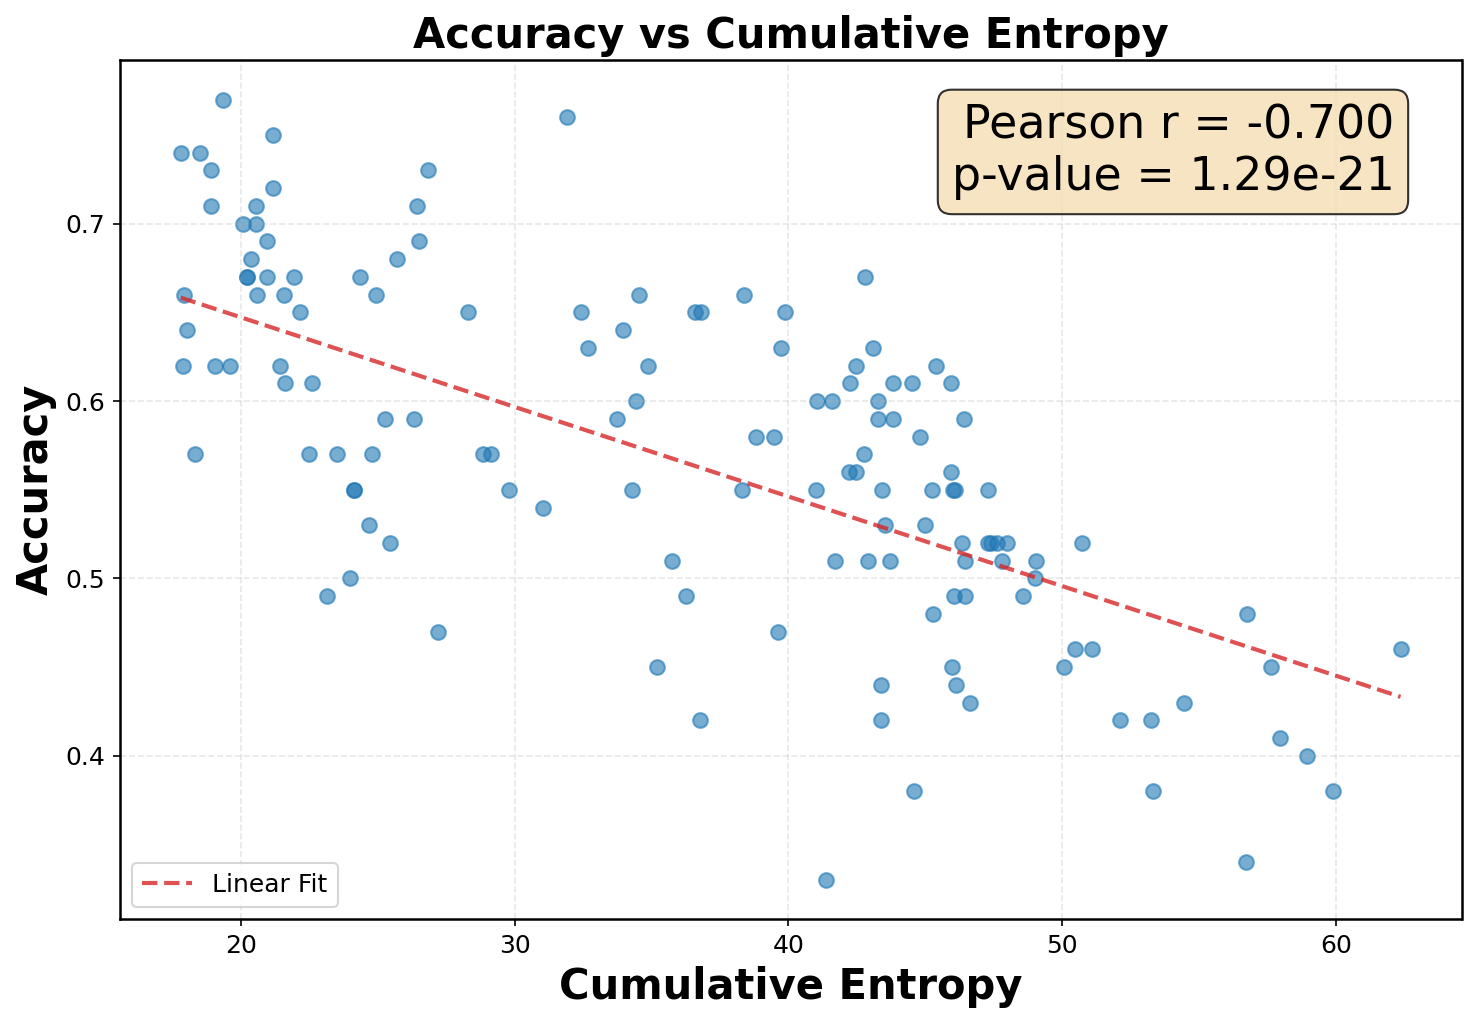
\includegraphics[width=1\linewidth]{image.png}
    \caption{topk-margin: temperature vs cum-entropy}
    \label{fig:placeholder}
\end{figure*}
\begin{figure*}
    \centering
    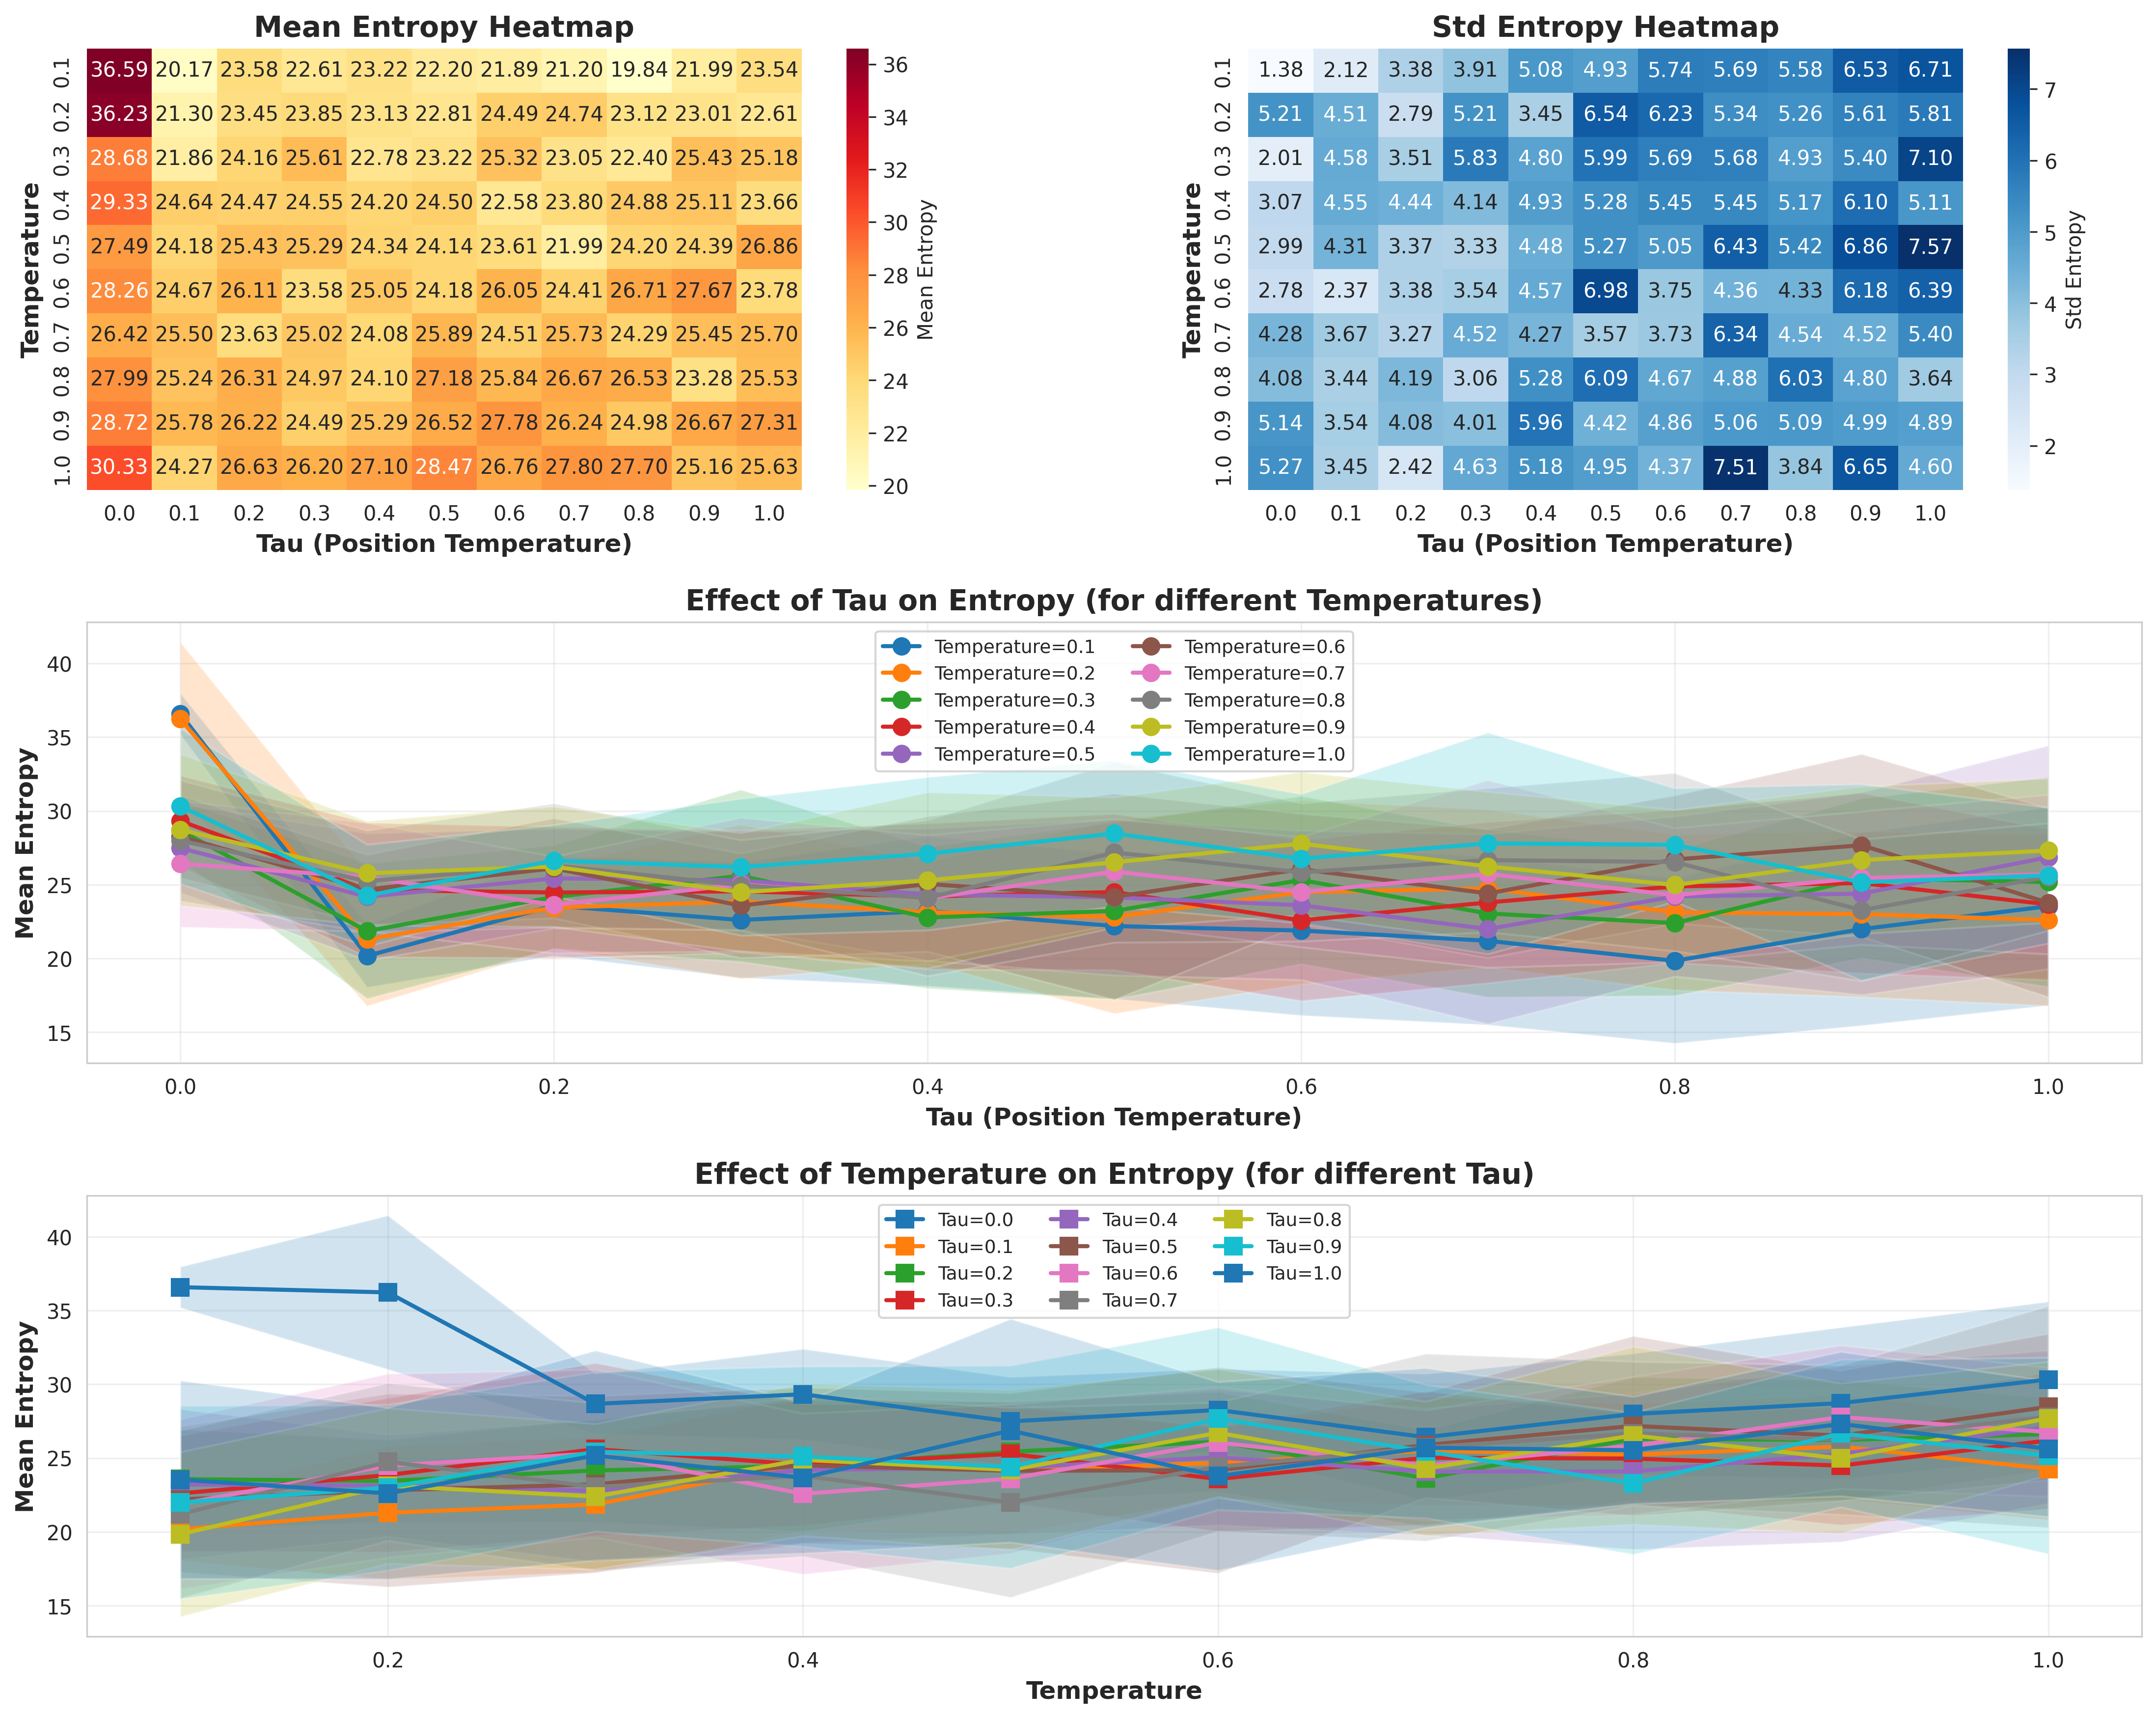
\includegraphics[width=1\linewidth]{ours-entropy-vs-temp.png}
    \caption{IGP: temperature vs cum-entropy}
    \label{fig:placeholder}
\end{figure*}
\begin{figure*}
    \centering
    \includegraphics[width=1\linewidth]{entropy vs acc.png}
    \caption{small budget calculation}
    \label{fig:placeholder}
\end{figure*}
\begin{figure*}
    \centering
    \includegraphics[width=1\linewidth]{acc-vs-cum-entropy.png}
    \caption{accuracy vs cumulative entropy}
    \label{fig:placeholder}
\end{figure*}

\begin{figure*}
    \centering
    \includegraphics[width=1\linewidth]{entropy vs temperature.png}
    \caption{cumulative entropy vs temperature}
    \label{fig:placeholder}
\end{figure*}

\begin{figure*}
    \centering
    \includegraphics[width=1\linewidth]{acc vs temperature.png}
    \caption{}
    \label{accuracy vs temperature}
\end{figure*}
\begin{figure*}
    \centering
    \includegraphics[width=1\linewidth]{alpha scheduler.png}
    \caption{alpha scheduler}
    \label{fig:placeholder}
\end{figure*}

% 讨论：K的效果
% 讨论：Focus的效果
% 讨论：Approximation的效果

% 一般来说performance和采样中的Stochasticity是反相关的。
% 但是在我们的算法中，并非如此。
% 1. 【PLOT】 entropy/maskgit_plus/topk_margin的 cumulative entropy vs temperature 图
% 2. 【PLOT】 temperature vs acc 图（用simple加减法来试试）
% 3. 【PLOT】 cumulative entropy progress。
% \subsection{Baselines}
% position sampler + heuristic selector + token sampler:
% [Scaling diffusion language models via
% adaptation from autoregressive models;
% MaskGiT;
% Topk-margin:
% Trainfortheworst,plan
% forthebest:Understandingtokenorderinginmaskeddiffusions]
Related works:
1. entropy
2. confidence
3. margin
4. PC-sampler
5. P2
6. uniform
7. KLASS
8. DUS

few features:
1. introduce position bias ?
2. kv cache ?
3. position stochasticity ?
4. 